\section{Delayed Acoustics Model}

Investigating the physics of of a thermoacoustic interaction requires the resolving of the full non-linear acoustics in the combustion system -- this might typically be a plenum, inlet, combustor and exhaust -- as well as the highly local reaction and diffusion phenomena located at the flame. In the case of a deflagration in a tube, the acoustics span the whole tube and a premixed flame and surrounding hydrodynamics will be located in one relatively small region of this tube. It would be natural, then, to fully resolve the flame and hydrodynamics by a fully simulated region and leave the which are the dominant effect upstream and downstream of the flame to be modelled separately. Assume at the simulation inflow that we can decompose the pressure and velocity fields as $u = \overline{u} + u'$ and $p = \overline{p} + p'$, where $\overline{\cdot}$ represents the average field at the inflow and $\cdot'$ represents fluctuations with zero mean. Then the value of $\overline{u} \pm c$ determines the speed of acoustic waves through the tube. Under a linear assumption for these acoustics -- i.e. the assumption that $ρ = \overline{ρ}$ such that $ρ' = 0$ or equivalently that acoustics do not interact with each other -- then the convection of an acoustic wave in a headwind and tailwind will cancel out. This results in a representative time delay $τ$ for the acoustic wave to leave the simulation domain, travel a distance $l$ both ways up- or downstream, and reenter:
\begin{equation}
τ = \frac{l}{c + u} + \frac{l}{c - u} = \frac{2l}{c} \, \frac{1}{1 - \Ma} \approx \frac{2l}{c}
\end{equation}
since under the deflagration approximation $\Ma \ll 1$. This is the time delay we will associate with the simulation inflow and outflow to represent their length scale via the delayed reentry of these acoustic into the inflow and outflow after a delay $τ_{\rm{U}}$ and $τ_{\rm{D}}$ respectively. This solves the linear acoustic problem in the tube upstream and downstream of the flame to leading order in Mach number. We refer to this non-DNS domain by the acoustic or fictitious domain or region.

\begin{figure}[t]
\centering
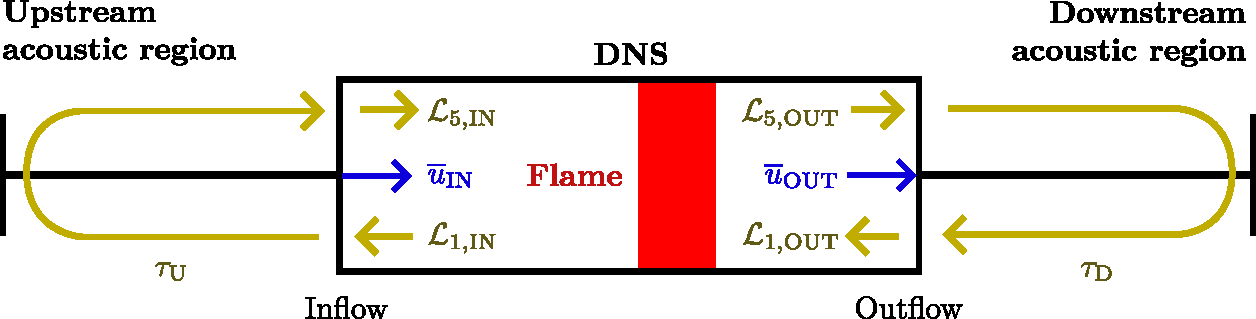
\includegraphics[scale=0.65]{assets/imgs/delay_bc_model.pdf}
\caption{Simple diagram for the simulation model.}
\label{fig:delay-model}
\end{figure}

To fit this model into the existing characteristic boundary formulation provided by NSCBC and LODI, we assume that we can store all of the outgoing acoustics as $\cl{L}_{\text{outgoing acoustic}}(t, \vb{y})$ where $\cl{L}_{\text{outgoing acoustic}}$ is the continuous outgoing field and the vector $\vb{y}$ parameterises the given connected inflow or outflow (this is a scalar value $y$ for 2 dimensional problems with vertical inflow or outflow). For a rectangular two-dimensional horizontal tube, this becomes $\cl{L}_{1/5}(t, y)$ where the outgoing acoustic is $\cl{L}_{1}$ for left-side boundaries and $\cl{L}_{5}$ for right-side boundaries (inflows and outflows respectively in this report). A simple diagram of the acoustic behaviour is shown in \fig{fig:delay-model} as acoustic values leave and reenter the DNS domain repeatedly. Continuing with this two-dimensional example, we would impose the delayed acoustic reentry by imposing at the left-side inflow that $\cl{L}_{5}(t, y) = \cl{L}_{5, \rm{nonreflect}}(t, y) + \cl{L}_{1}(t - τ, y)$ where the first term $\cl{L}_{5, \rm{nonreflect}}$ is the required condition described in the previous chapter to stop the outgoing acoustic from being immediately reflected. Under this model, we are implicitly assuming each location at the boundary has its own one-dimensional acoustic approximation being made. For the rest of the report we instead use a simpler formulation which averages the acoustics across the boundary as they leave:
\begin{subequations}
\begin{equation} \label{eqn:L-delay-form}
\cl{L}_{5}(t, y) = \cl{L}_{5, nonreflect}(t, y) + \langle \cl{L}_{1}(t - τ_{\rm{U}}, \cdot\,) \rangle_{\rm{IN}}
\end{equation}
for inflows and
\begin{equation}
\cl{L}_{1}(t, y) = \cl{L}_{1, nonreflect}(t, y) + \langle \cl{L}_{5}(t - τ_{\rm{D}}, \cdot\,) \rangle_{\rm{OUT}}
\end{equation}
\end{subequations}
%(NOT SURE WHAT TO DO IF THESE WAVES DO NOT FULLY REFLECT?)
for outflows, where $\langle\,\cdot\,\rangle_{\rm{IN/OUT}}$ represents averaging over inflow or outflow boundary values respectively. This corresponds to a single one-dimensional approximation being made for each boundary, which is of course only valid for thin-enough computational domains. We refer to these boundary conditions as \emph{Acoustic Delay Characteristic Boundary Conditions} (ADCBC).

Since we are modelling the reaction Navier-Stokes equations, we must also impose that all other incoming $\cl{L}$ values vanish at the inflow so that no entropy, shear or mass waves enter the domain. Note that now no relaxation terms are used on either boundary -- this marks the main difference between ADCBC and NSCBC. Relaxation terms are traditionally used under the NSCBC formulation to ensure the dependent variables -- inflow velocities $\vb{u}=(u, v)$, temperature or density and mass fractions and especially outflow pressure -- do not drift as characteristic waves leave the domain, not to return under perfectly non-reflecting conditions. Given that the acoustic waves will be returning under ADCBC, we do not need these relaxation terms for inflow normal velocity ($u$ in our vertical boundaries) or outflow pressure as they are closed by the full reflection of these acoustic waves. Note that if relaxation terms were imposed on top of the delayed reflections, we would be applying a further well-posing condition to a problem which is already well-posed. For the other variables, relaxation terms may be kept, but we have chosen to remove them under the assumption that the simulation is strongly one-dimensional and inert at the boundary. That is, no significant shear, entropy or mass waves should be leaving these boundaries, so the related dependent variables $v$, $T$, $Y_α$ will not drift. All that is left is to apply the diffusive BCs as the remaining physical BCs. Nothing here changes with \cite{sutherland2003ImprovedBoundaryConditions}, where they use the zero normal flux conditions \equ{eqn:znf}. A further consideration to make is what happens when the acoustic field is strong enough that $\abs{\overline{u}} < \abs{u'}$ at the inflow or outflow. Usually we expect this to happen at the inflow first since $\abs{\overline{u}_{\rm{IN}}} > \abs{\overline{u}_{\rm{OUT}}}$, i.e. the acoustic field has become large enough that the inflow has become an outflow at the left side of the domain. To account for this, we simply check if the sign of $\vb{u}\cdot\uvec{n}$ at this boundary where $\uvec{n}$ is the outward pointing normal and apply the conditions for $\cl{L}$ and diffusion correspondingly.

To outline the method once more, we will be introducing a delay for acoustics leaving the simulation domain to model an extended acoustic domain which is not a part of this acoustic region. This will be done using non-reflecting characteristic boundaries and storing the acoustics which leave the domain. These acoustics are then simply reintroduced after the relevant time delay.

Later on, these definitions for $\cl{L}_{1/5}$ can be extended to include an imposed acoustic field if that is desirable, e.g. to simulate a secondary thermoacoustic instability response. Furthermore, this method could also be extended to arbitrary numbers of delay boundaries with any boundary normal, although modelling a physical geometry in this way would be a challenge which is not explored in this work.




\section{Implementing the Model}

The SUNSET code, like other CFD codes, uses a discretised temporal domain to integrate forward in time. Hence, we already only have access to the outgoing characteristics at discrete time steps and cannot recover the exact value of $\cl{L}_{1}(t - τ, y)$ when $t - τ$ does not lie on a previous time step, assuming a left-side boundary. On top of this, the step size taken by a typical combustion simulation is likely to oversample the acoustic field at the boundary, resulting in a much higher memory footprint that is required by the method. This, along with the variable time steps used in the SUNSET code means we aim for a sample rate $δt_{\rm{sample}} > δt > 0$ for these $\cl{L}_{1}$ values. We refer to the sample times and acoustics as $\{(t_s, \overline{\cl{L}}_{1, s})\}_{s=1}^{N_{\rm{samp}}}$ where $s\in\bb{Z}$ enumerates these sample times so $t_{N_{\rm{samp}}}$ is the most recent sample time and $\overline{\cl{L}}_{1/5, s} \equiv \langle \, \cl{L}_{1}(t_s, \cdot\,) \, \rangle_{\rm{IN}}$. To evaluate the $\langle \cl{L}_{1}(t - τ_{\rm{U}}, \cdot\,) \rangle_{\rm{IN}}$ term on the right-hand side of \equ{eqn:L-delay-form}, we simply interpolate between values of $(t_s, \overline{\cl{L}}_{1, s})$ at the interpolated time $t' \equiv t - τ_{\rm{U}}$. Note that no requirement is made here that this interpolation conserve the acoustic energy which left the domain. If significant acoustic losses or gains are made as a result of this, an acoustically conservative method should later be investigated.


\subsection{Code Schematic}

Since the time delay is only a finite length, clearly the oldest sample values we expect to need are $\cl{L}_{1}(t', \cdot\,)$ where $t' \approx t - τ - δt_{\rm{sample}}$. Hence, we only need to store the finite number of samples $\bb{T} \cross \bb{L} = \{(t_s, \overline{\cl{L}}_{1, s}) \, : \, t_s \in [t - τ - δt_{\rm{sample}}, t]\}_{s=1}^{N_{\rm{samp}}}$ at any given simulation time $t$. For as long as $τ$ remains bounded, the size of $\bb{T} \cross \bb{L}$ -- and hence our memory footprint -- also remains bounded. Thus far, we have assumed that the up- and downstream tube lengths $l_{\rm{U/D}}$ remain constant, but they may actually change arbitrarily alongside their associated time delays $τ_{\rm{U/D}}$ provided it does not exceed the sound speed, so multiple acoustics do not reenter the domain at one sample time. Having said that, as long as we know the maximum delay time $τ$ occurring in a given simulation, we can store $\bb{T} \cross \bb{L}$ in a contiguous portion of memory which the delay boundaries are allocated at the beginning of the simulation. This is done using a one-sided queue data structure, which is implemented as a \emph{first-in, first-out} (FIFO) wrapper around a contiguous array. In this way, samples from the current simulation time may be added to the end of the queues and values which are needed for interpolation are found at the beginning of the queue. Once they are no longer needed for an accurate interpolation of $\cl{L}_{1}(t', \cdot\,)$, they are \emph{popped} (removed) from the beginning of the queue. If some other data structure was used instead for these samples, then the data would slink through memory in a way where \emph{contiguity} cannot be enforced for arbitrary simulation times. Note that a linked list would be subject to this issue, be slower to traverse for interpolation values and provide $\cl{O}(1)$ deletion of random samples, which we do not require here.

\begin{figure}[t]
\centering
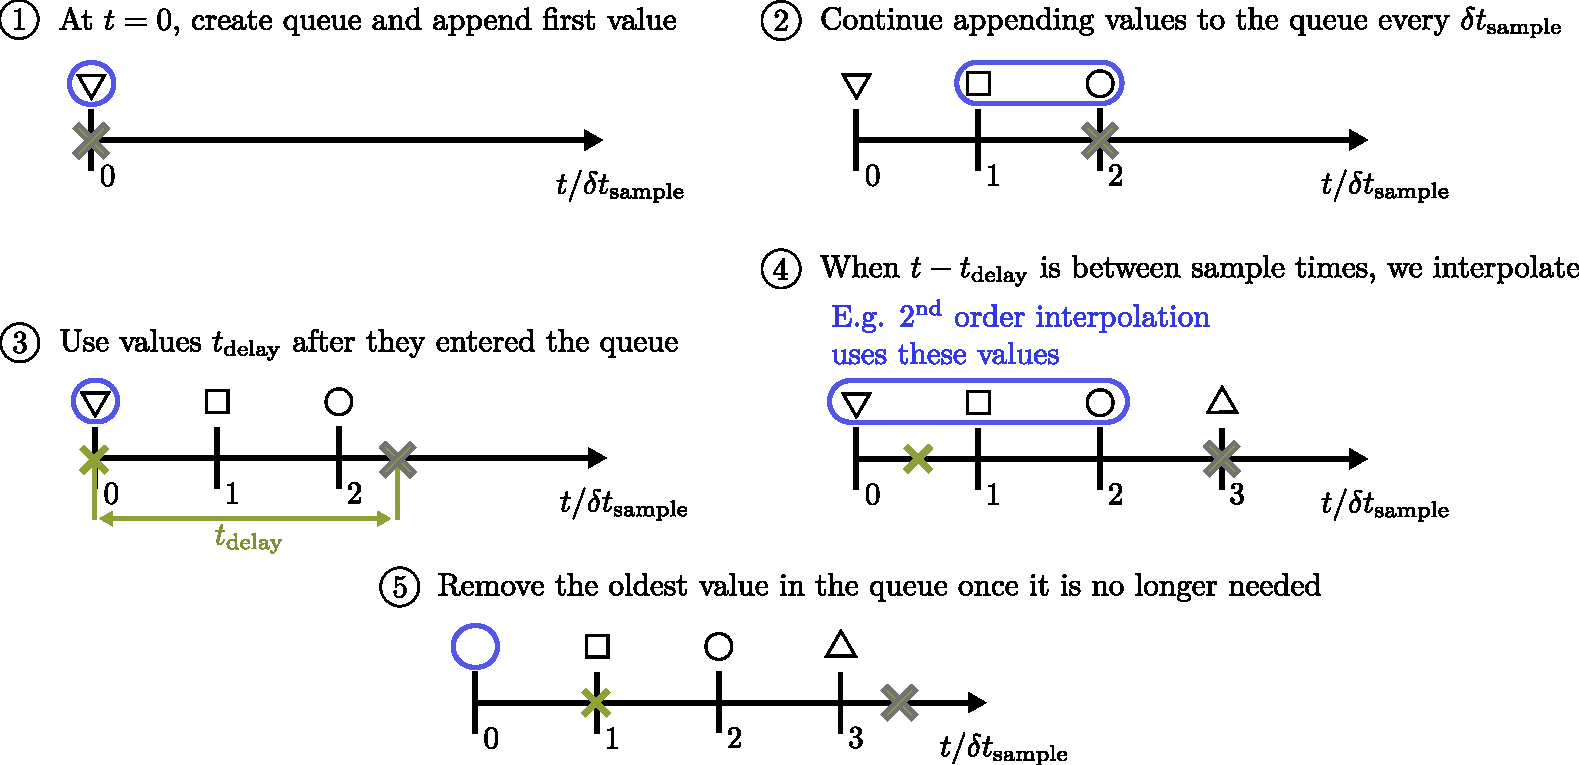
\includegraphics[scale=0.65]{assets/imgs/delay_bc_queue.pdf}
\caption{An illustration of how this queue system is used for boundary sampling. Different shapes are used to represent the different values in $\bb{T} \cross \bb{L}$. The values relevant to the current step is circled in blue.}
\label{fig:delay-queue}
\end{figure}

This queue system is illustrated in \fig{fig:delay-queue} in a continuous temporal domain for simplicity so sample times remain uniformly spaced. The first two steps, (1) and (2) show values being appended to the queue at the beginning of the simulation until the time delay is reached in the third step, (3). The fourth step, (4) shows which values are used for interpolation in an example second order interpolant. The fifth and final step, (5) shows old values being removed from the start of the queue.

\begin{figure}[t]
\centering
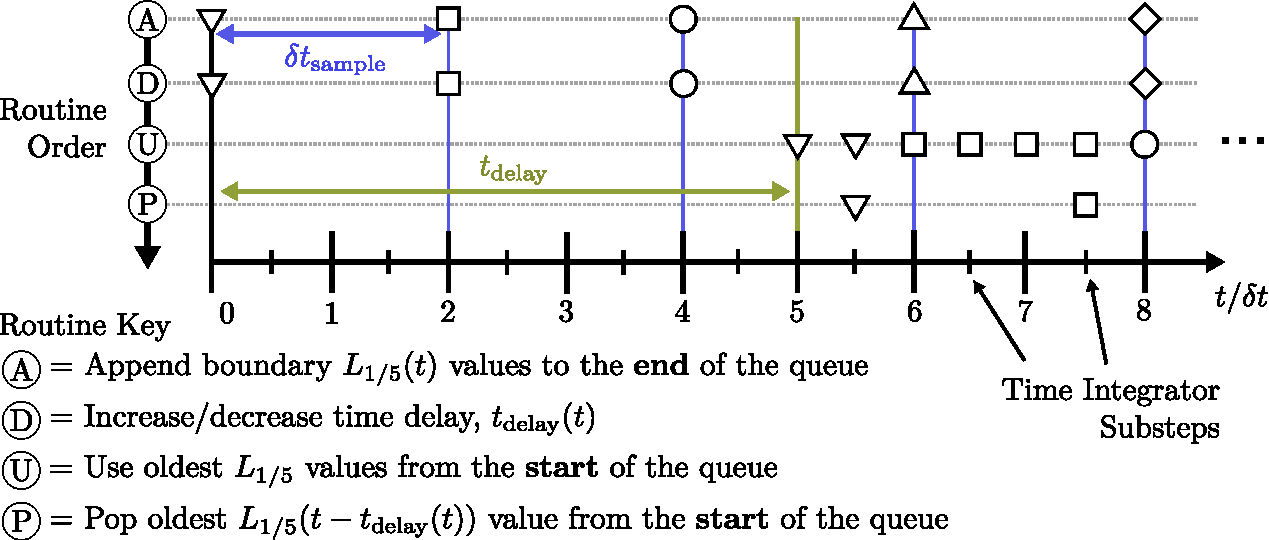
\includegraphics[scale=0.65]{assets/imgs/delay_bc_code_schematic.pdf}
\caption{Routine schematic for ADCBC implemented into a time integrator with two substeps. A sample period $δt_{\rm{sample}} = 2δt$ is used in this example. The evaluation of routines (or procedures) are shown in order from top to bottom (starting with (D) and ending with (U), key given in the figure), left to right (beginning at $t = 0$ and showing up to $t = 8 δt$). A routine being used is signified by a shape representing given sample in $\bb{T} \cross \bb{L}$. The time delay $τ \approx 4 \frac{3}{4} δt$ is shown in gold.}
\label{fig:schematic}
\end{figure}

\fig{fig:schematic} illustrates the full schematic for a time integrator with two substeps per time step and uniform time step size. Sampling is performed in the routine (A) which is called every sample time preceded by a change to $τ$, if required. These are circled and labelled (1) and (2) corresponding to the steps in \fig{fig:delay-queue}. Only after the full time delay $τ$ do the values from the beginning of the queue start to get used in the routine (U). This is shown in the labels (3) and (4) corresponding to those steps in \fig{fig:delay-queue}. Finally, step (5) removes the oldest value from the queue only once they are not needed in the routine (R). Appending and removal from the queue happen before the queue values are used for interpolation to ensure the correct values are available in the queue for interpolation. Note that the routine (U) happens every substep using as many values from the beginning of the queue as are required. The shape shown for this routine in steps (3) and (4) are just the earliest sample taken which would be used.



\subsection{Memory Footprint}

The obvious disadvantage of this ADCBC method is the potential size of queues required to hold the data in $\bb{T} \cross \bb{L}$. This data should only be available to those processors relevant to the boundary nodes, so the memory burden should be held by those processors alone, since the SUNSET code is ran as a distributed system, where memory is allocated to each processor separately. If the memory footprint is too large ($\cl{O}(1~\rm{GB})$ for modern hardware), then the simulations will likely crash and high-memory compute nodes would be required. This is to be avoided. Let us now perform a simple calculation to estimate the memory required by a given acoustic delay characteristic boundary. Assume $l = 1$ m, $c = 343$ m s$^{-1}$ and that a typical sample period is approximately $δt_{\rm{sample}} = 10^{-7}$ s (this will be validated in the coming chapter). Then, the number of numbers which need to be stored in memory are:
\begin{equation}
N_{\rm{numbers}} = 2 \frac{τ}{δt_{\rm{sample}}}
= \frac{4 l}{c δt_{\rm{sample}}}
\approx 1.17 \cross 10^5.
\end{equation}
For double precision floating point numbers, these require 8 bytes of storage each, resulting in $9.33 \cross 10^5$ bytes $\approx 1$ MB. This can easily be stored and accessed on modern memory, albeit may not be stored in the processor's cache. This is not a concern as remaining memory required by the LABFM discretisation dwarfs this.

In a separate formulation where acoustics across the boundary are not averaged and instead we have separate queues for samples taken at each boundary node, we are likely to have less than 100 boundary nodes per processor in two-dimensions (and fewer or the same in three). This results in a 100 MB memory requirement, which is still manageable. If longer, e.g. $l = 10$ m, domains are modelled, then this could become a significant issue. Importantly, the total memory requirement under this method is significantly lower than if you had discretised the fully non-linear acoustics in the up- and downstream regions, but these discretisations would be easier to decompose into separate processors. The potential issue then, comes from the fact that this memory burden is placed only onto the boundary nodes, which would have less memory available than the total memory provided in a theoretical decomposition of the acoustic region between more processors.




